% Created 2012-11-12 Mon 15:26
\documentclass[11pt]{article}
\usepackage[utf8]{inputenc}
\usepackage[T1]{fontenc}
\usepackage{graphicx}
\usepackage{longtable}
\usepackage{float}
\usepackage{wrapfig}
\usepackage{soul}
\usepackage{amssymb}
\usepackage{hyperref}


\title{SiconosMechNotes}
\author{jan michalczyk}
\date{12 November 2012}

\begin{document}

\maketitle

\setcounter{tocdepth}{3}
\tableofcontents
\vspace*{1cm}

\section{First meeting on <2012-10-26 Fri> in Grenoble}
\label{sec-1}


\subsection{General objective's outline}
\label{sec-1.1}


   Project's objective is to elaborate in terms of both design and implementa-
   tion a library for multibody systems simulation - SICONOS MECHANICS.
   Designed solution will be based on already developed SALADYN project.
   In essence, the goal is to enhance SALADYN by equipping it with more
   functionalities such as: collision detection engines from already existing li-
   braries like PhysX/Bullet (used by TRASYS in 3DROV), CAD, geometry
   and visualization capabilities from OpenCASCADE and FreeCAD, models
   description using XML language or Python scripting in order to avoid hav-
   ing to define them in C++ from the front-end side. The use of a reliable
   collision detection library coupled with SICONOS as computation engine is
   expected to provide a simulation environment for multibody systems where
   contact phenomena are taken into account. Up to now such tool does not
   exist. Thus, an expected outcome will be a more complete simulation tool
   for multibody systems using SICONOS Kernel and Numerics as contact sim-
   ulation engine interconnected with other tools as shown on the figure below.
   As displayed on the figure, there are different tools available as for example
   ROS parser for urdf files which might be used in order to generate robot
   model equations replacing HuMAns and Maple. Furthermore, urdf file for-
   mat allows the exportation to Gazebo robot simulator where also a controller
   can be designed and visualization can be achieved. Models can be described
   in Python at front-end and thereafter parsed into urdf format. Coherence
   between the used mathematical formalism in expressing the dynamics of the
   system and the formalisms used in the aforementioned libraries (i.e. Bul-
   let/OpenCASCADE) needs to be assured on the level of API.
   
 
   \begin{figure}[htb]
\centering
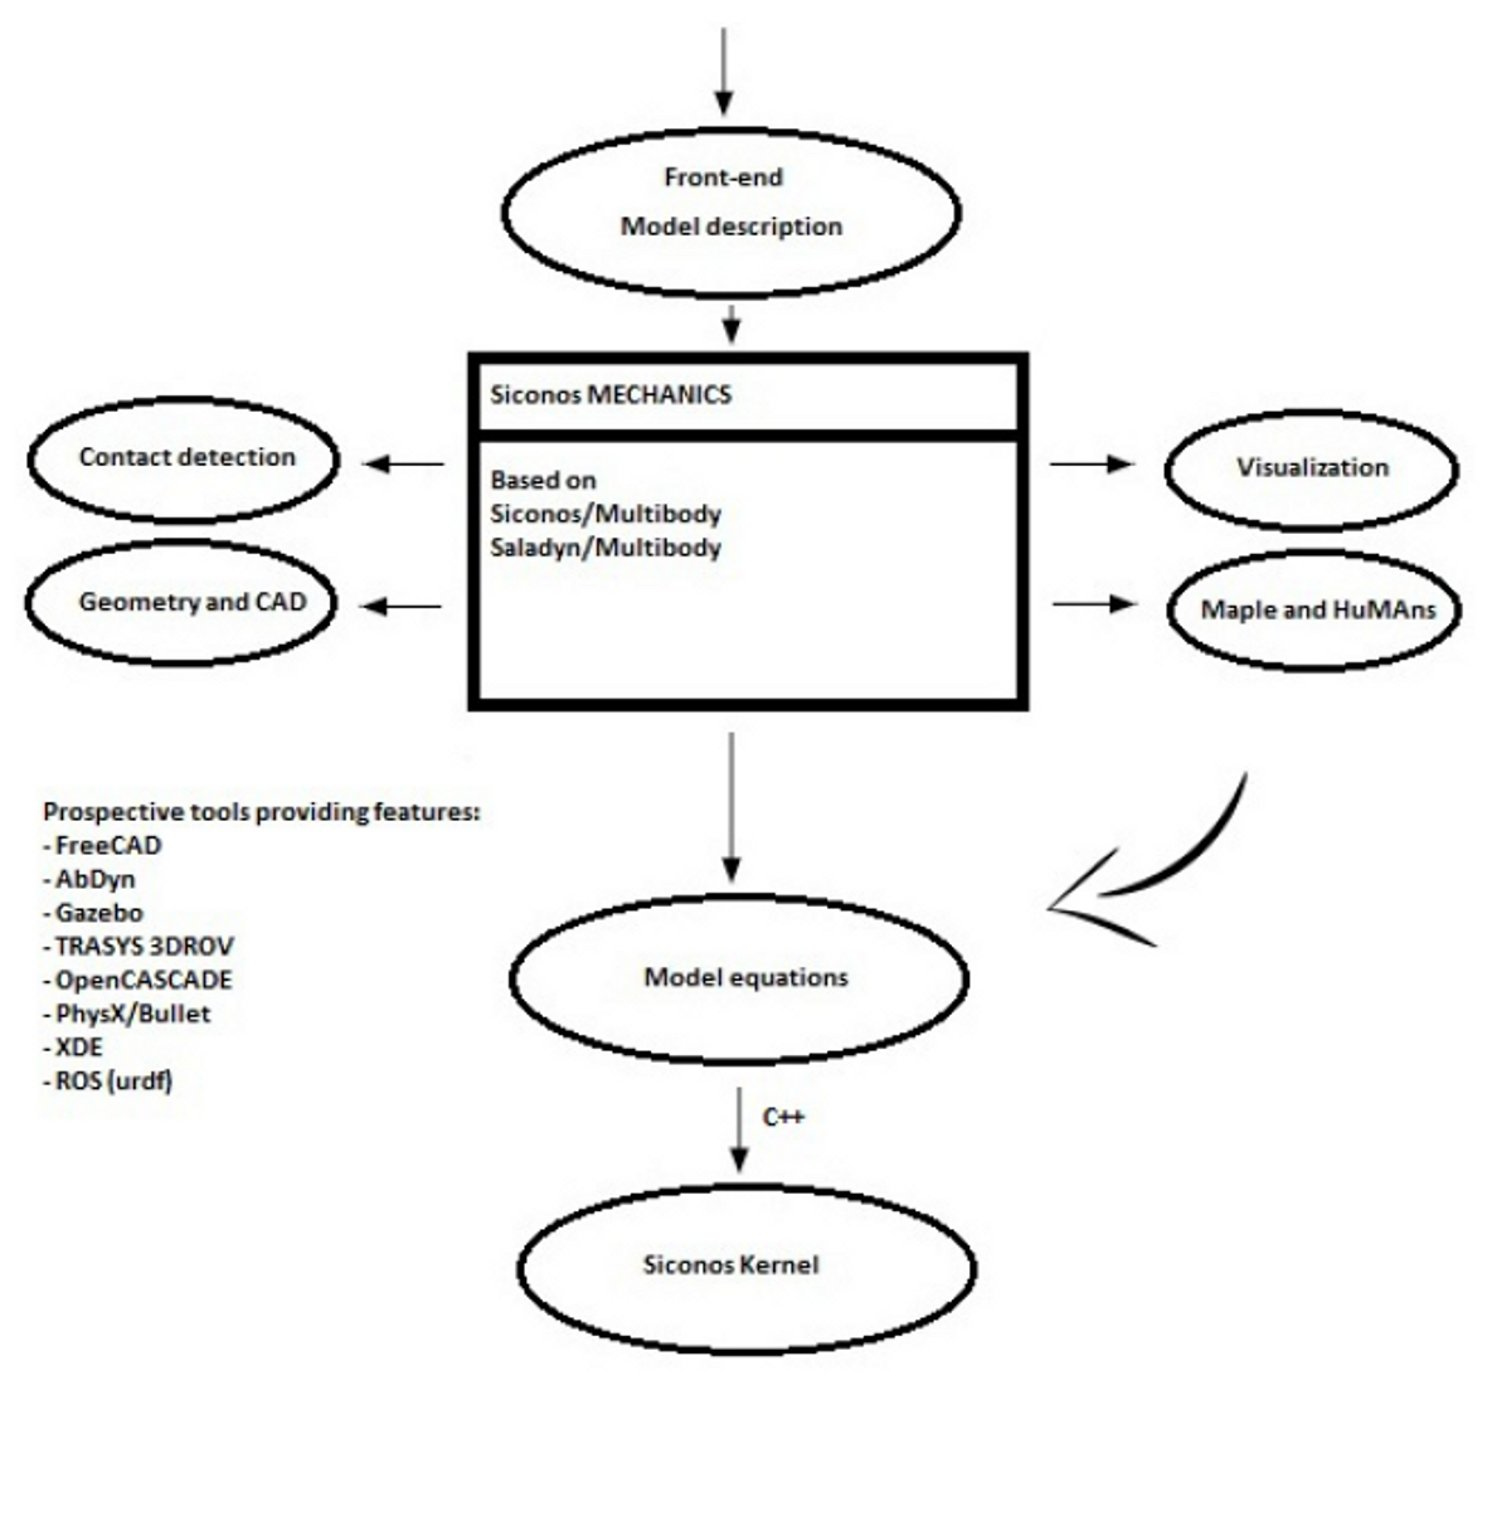
\includegraphics[width=10cm]{./scheme.jpg}
\caption{\label{fig:fig1}Functionalities scheme}
\end{figure}

   An important aspect of the short-term project timespan is a survey on existing tools 
   which provide the above listed features. Among ones already mentioned are:
   MbDyn library, Gazebo, ROS.

\subsection{Timespan of planned work for next weeks}
\label{sec-1.2}


\subsubsection{Get familiar with SICONOS}
\label{sec-1.2.1}


\begin{itemize}
\item Examine the ``Bouncing Ball'' example
\item Examine the ``double Pendulum'' example as an example requiring the use of plug-ins
\item Expected duration: 2 weeks
\end{itemize}
\subsubsection{Exammine and upgrade the "Rover" example}
\label{sec-1.2.2}


\begin{itemize}
\item Examine its relation with HuMAns software (equations generation)
\item Generate the triangle mesh as a ground for new simulation
\item Run the simulation on the previously generated triangle mesh
\item Expected duration: 3 weeks
\end{itemize}
\subsubsection{Examine the purposefullness of using Bullet library for collision detection}
\label{sec-1.2.3}


\begin{itemize}
\item Use collision detection from Bullet in the ``Rover'' example
\item Duration: undefined
\end{itemize}
\subsubsection{Examine SALADYN an OpenCASCADE}
\label{sec-1.2.4}


\begin{itemize}
\item Link SALADYN and openCASCADE
\item Duration: undefined
\end{itemize}
\subsection{Additional remarks}
\label{sec-1.3}


   Meetings will be held every second week to assure the right progress
      

\section{Second meeting on <2012-11-09 Fri> in Grenoble}
\label{sec-2}


\subsection{First important point - theoretical background on collisions}
\label{sec-2.1}


   The meaning of different coordinate systems transformations is crucial in understanding
   and implementing numerically an algorithm for an interaction of a wheel (or other object)
   with a plane. Let's consider that situation in details on the example of a manipulator arm
   colliding with a motionless rigid body.


   \begin{figure}[htb]
\centering
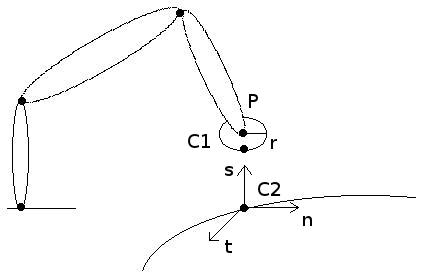
\includegraphics[width=10cm]{./contact.jpeg}
\caption{\label{fig:fig2}Collision between two rigid bodies}
\end{figure}
   
  
   In this situation one has a geometric robot jacobian which maps the joint-space velocity
   into the velocity of the end-point (or any other point in the kinematic chain).
   One calculates this jacobian by taking the derivatives of cartesian coordinates of 
   end-effector (which are functions of generalized coordinates given by the forward
   kinematics) with respect to generalized coordinates. For the purposes of simulation we
   need to calculate the distance between the end-effector and the plane. We do that to be
   able to detect the moment when the constraint is being violated (impact occurs).
   When dealing with impact one has to know the velocity of the impacting body with respect
   to the local frame (the frame consisting of the plane and the normal to the plane in the
   point of impact). This velocity is needed by the Newton's impact law. The local frame is
   where the contact point is - this is very important as we will have to transform the 
   velocity of the end-effector expressed in the global frame into the velocity relative 
   to the plane (expressed in the local frame). Therefore we need to establish a new 
   transformation matrix between the local and global frames. This new transformation 
   maps global (cartesian) velocity of the end-effector into the velocity in the local frame. 
   This operator will also be used to transform the contact forces into the generalized 
   forces in robot joints. That is because contact forces are always expressed in the local 
   frame defined in the contact point. 
  
\subsection{Detailed description of the algorithm}
\label{sec-2.2}

  
\subsubsection{Distance calculation}
\label{sec-2.2.1}


    We project the point in space on each of the planes defined by each of the traingles.
    In this way we create as many interactions as there are wheels times the number of
    triangles. This is not the most efficient method but it will be the first attempt.
    In the next attempt a space filter should be used which will discard the triangles
    with which a wheel has no possibility to enter in contact. 
    After projection on the plane there is a possibility that either point lies inside the 
    triangle or outside of it. If it lies inside then there is no problem and we calculate
    the distance between the point and the plane.
    If it lies outside of the triangle we need to be able to 
    calculate the distance nevertheless. Therefore, we calculate the distances from the 
    lines defined by the edges of the triangles, we take the line we are closest to and
    then we check if the projection of the point on that line lies within the edge.
    If it does then we take the distance as the distance between the point and its projection
    on the edge. However if the point lies outside of the segment (edge), then we calculate
    to which of the two vertices (points at each end of the edge) the projection is closer.
    Finally, we take as the distance we're looking for a distance between this vertex and 
    the projection of the given point.
    When calculating the normal to the contact point, we take the normal to the same 
    plane regardless of the feature we calculated the distance to (vertex, plane, edge).

\subsubsection{Calculation of the normal to the plane and the local coordinate frame}
\label{sec-2.2.2}


    Once the distance function assumed zero value, it means that the contact occured.
    Then we should proceed to calculate the local coordinate frame in the contact point. 
    We will need it to have the rotation matrix from global frame to the local one.
    We can compute the normal by taking the cross product of two vectors defining the plane.

\subsubsection{Calculation of the contact jacobian}
\label{sec-2.2.3}


    Contact jacobian can be calculated as follows (assuming the local frame is not moving):
    \begin{equation}
    v_{c_{1}} = -R^{-1}J(q)\dot{q}
    \end{equation}
    Where:
    \begin{equation}
    -R^{-1}J(q)\dot{q} = G
    \end{equation}
    Which is a contact jacobian we're looking for. Inverse of that jacobian allows to obtain
    velocities and forces after impact.
    
\subsection{Activities}
\label{sec-2.3}


\subsubsection{\textbf{TODO} Terrain generation}
\label{sec-2.3.1}


    I should generate a static terrain with some fixed area filled with triangles with some 
    elevation. This terrain will initialize the terrain in C++ code used for simulation.
    That is to say, values read from VRML or .DEM file will initialize abstract objects in
    C++. Terrain should be generated in .DEM file or the file format imposed by Trasys. 
    The keypoint is to be able to initialize from this format the values of objects in C++
    (plane coefficients and other values needed for computations).
    Each triangle from the map will instantiate one relation (one trinagle forms one constraint
    plane). There will be six sets of relations representing constraint planes - one for
    each wheel.
    There should be also a way to visualize the content of the file
    (there are methods to convert .DEM into VRML).
    
\subsubsection{\textbf{TODO} Relation definition}
\label{sec-2.3.2}


    With respect to what has been exposed in teh first section in the relation class I need
    to provide methods to calculate distance according to the algorithm described above, as
    well as Jacobian transforming velocities and forces from local into global frame.
    A class representing relation plane-wheel needs to be written. This class will inherit
    from the class representing the scleronomous relation in SICONOS. Crucial methods in this
    class are: ComupteJacobianh() and Computeh().

\subsubsection{\textbf{TODO} Combine it alltogether, simulate and visualize the results}
\label{sec-2.3.3}

    
    In order to run the simulation the existing code will be reused.
    New relation class will be insterted into the main piece of code. Also, code reading in
    the initialization data for the relations from the VRML (or .DEM) file needs to be
    included in the main file.
    
    

\end{document}